
\chapter{Engineering and fabrication} 

%This chapter includes all the engineering and fabrication details
%needed to develop the product. 

\section{Product structure}
The product looks like a simple box from outside but it's more than that. Beneath the button is a speaker and beside it lies a microphone. Top panel is a 3D printed panel, housing emergency button, speaker and microphone. Bottom side of top panel takes care of connection between the custom build button assembly and a push button switch, provides support for speaker housing and a projection to press push button of tamper detection module. The base hosts most of the electronics. Half of the base part is occupied by raspberry pi and its add-on board, other half is occupied by the battery and its charging circuitry. Side wall of base part exposes power connector to charge the secondary battery and power the entire electronics. Figure~\ref{fig:block_dia} shows the block diagram of the complete design.\\
In this chapter, we look at hardware tools, software tools and assembly/fabrication procedures required to make \emph{PanicButton device}. 

\begin{figure}[H]
\centering
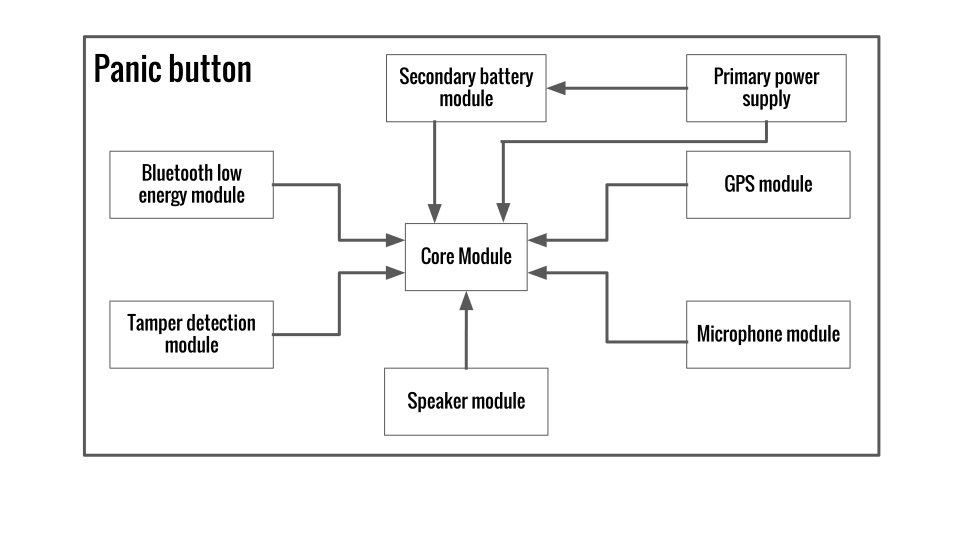
\includegraphics[width=\textwidth]{block_dia}
\caption{Block diagram of the \emph{PanicButton device}}
\label{fig:block_dia}
\end{figure}

%This section provides the overall structure of the product in a top-down
%manner as viewed by a person when opening up the product completely
%to its component parts. The overall structure is given with the help
%of a block diagram schematic. On some modules, embedded software may
%reside and its structure diagram can be shown separately module-wise.
%The structure diagram for any standalone software should also be included.


\section{Hardware modules}
The \emph{PanicButton device} can be divided into three parts namely raspberry pi, add-on board for raspberry pi and the enclosure. Base part of the enclosure acts the hosing for these modules.

\subsection{Raspberry pi}
Raspberry pi's sd card with modified Raspbian image, must be installed into the raspberry. Raspberry pi should be mounted on the base using four M2 screws of 0.5 cm length.

\subsection{Add-on board for raspberry pi}
Add-on board contains the BLE module, programming header for BLE module, GPS module, speaker module, emergency button headers and tamper detection module. Figure~\ref{fig:schematic} shows the circuit schematic for the raspberry pi's add-on board.

\begin{figure}
\centering
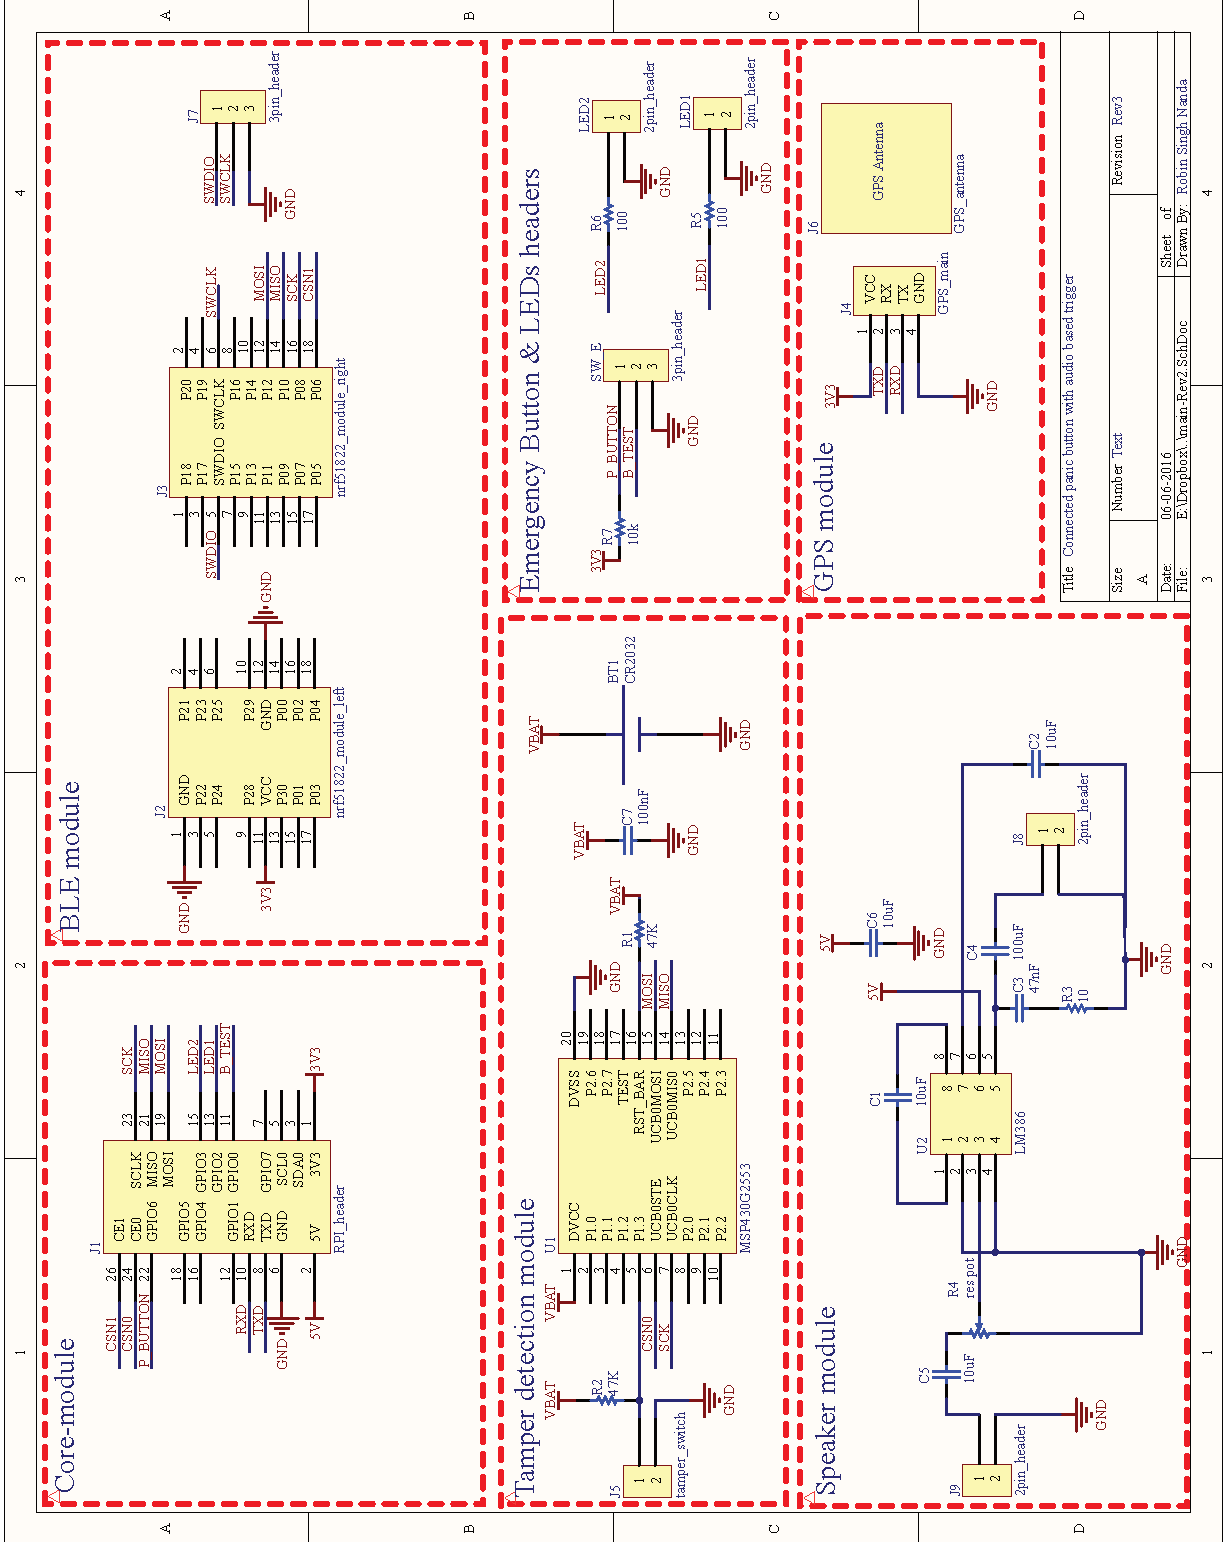
\includegraphics[width=\textwidth]{schematic}
\caption{Schematic of raspberry Pi add-on board}
\label{fig:schematic}
\end{figure}
The add-on board has a non rectangular shape because of the ethernet and USB connectors of the raspberry pi. Mounting holes of the add-on board are aligned to the mounting holes of the raspberry pi board. Figure.~\ref{fig:enc_top_view} shows the top layer of add-on board's PCB and figure.~\ref{fig:enc_bottom_view} shows the bottom layer of the add-on board's PCB. Our application did not impose any constrain on the thickness of the substrate, hence common substrate of 1.6 mm thickness was used. All signal tracks on the PCB are of 10 mil width. The add-on board connects to raspberry pi via 26 pin female header and can be secured using M3 mounting screws.

\begin{figure}[H]
\begin{subfigure}{.5\textwidth}
  \centering
  \includegraphics[width=.95\linewidth]{pcb_top}
  \caption{Top side}
  \label{fig:enc_top_view}
\end{subfigure}%
\begin{subfigure}{.5\textwidth}
  \centering
  \includegraphics[width=.95\linewidth]{pcb_bottom}
  \caption{Bottom side}
  \label{fig:enc_bottom_view}
\end{subfigure}
\caption{Top side and bottom side of PCB of Raspberry pi add-on board}
\label{fig:enc_views}
\end{figure}

Figure~\ref{fig:bom} shows the bill of materials used in this project.
\begin{figure}
\centering
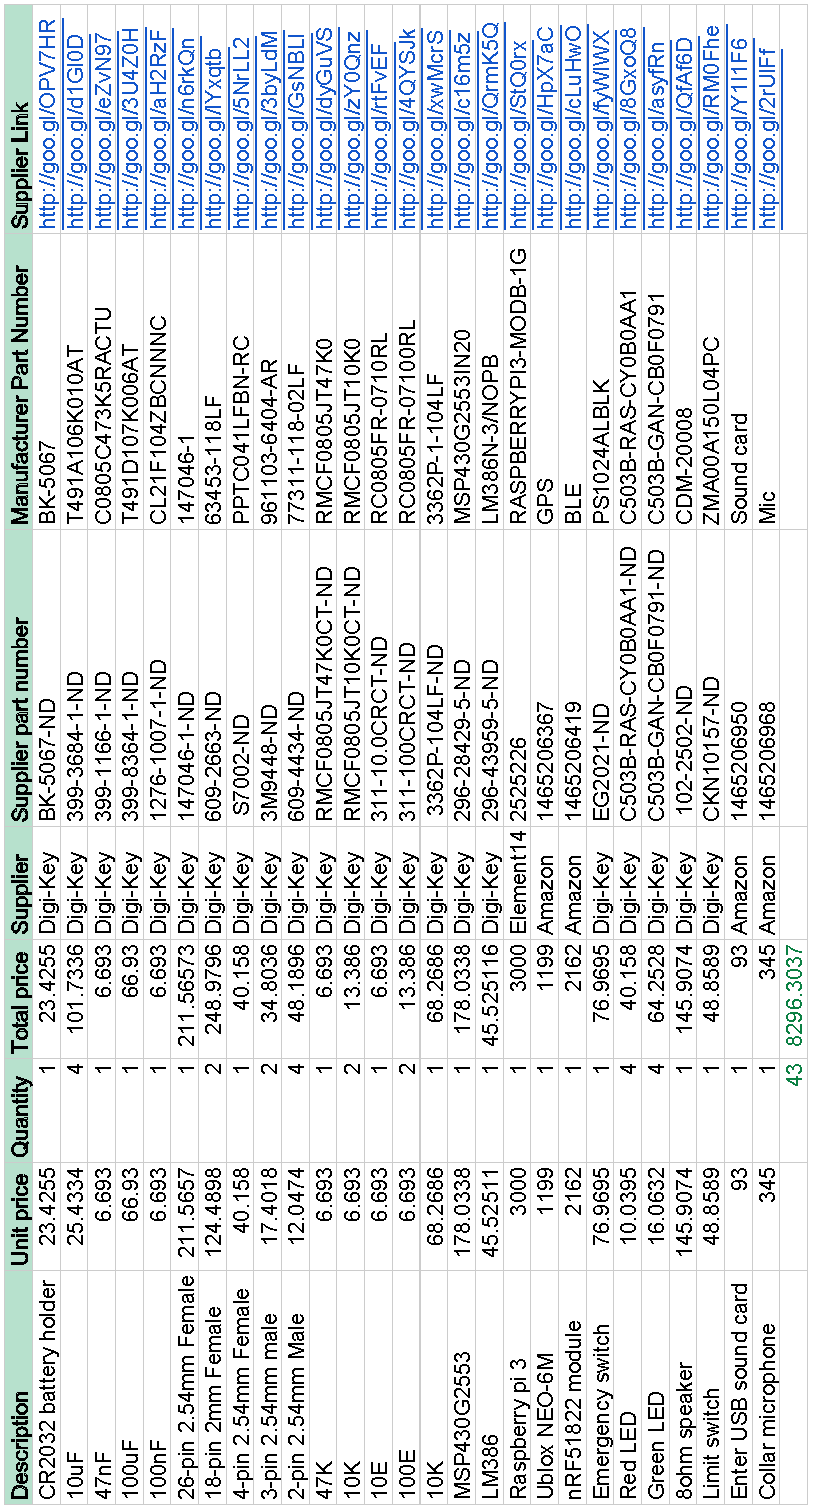
\includegraphics[width=0.8\textwidth]{bom}
\caption{Bill of materials}
\label{fig:bom}
\end{figure}
\subsection{Enclosure of \emph{PanicButton device}}
Enclosure was fabricated using a 3D printer that uses fused deposition modeling technique. Many parts of top panel were fabricated individually. Figure ~\ref{fig:enc_views} shows different views of the fabricated panic button enclosure. 

\begin{figure}
\begin{subfigure}{.5\textwidth}
  \centering
  \includegraphics[width=.9\linewidth]{enc_top_view}
  \caption{Top view}
  \label{fig:enc_top_view}
\end{subfigure}%
\begin{subfigure}{.5\textwidth}
  \centering
  \includegraphics[width=.9\linewidth]{enc_side_view}
  \caption{Side view}
  \label{fig:enc_side_view}
\end{subfigure}
\begin{subfigure}{.5\textwidth}
  \centering
  \includegraphics[width=.9\linewidth]{enc_side_view2}
  \caption{Front view}
  \label{fig:enc_side_view2}
\end{subfigure}%
\begin{subfigure}{.5\textwidth}
  \centering
  \includegraphics[width=.9\linewidth]{enc_iso_view}
  \caption{Isometric view}
  \label{fig:enc_iso_view}
\end{subfigure}
\caption{Different views of the enclosure}
\label{fig:enc_views}
\end{figure}

%For every hardware module, the following engineering and fabrication
%details should be included,
%\begin{itemize}
%\item physical dimensions with mounting hole details
%\item connectors and connector pin details with pin-level labeling
%\item circuit diagram using connector pin-level labeling as inputs and outputs
%\item printed circuit board layout with circuit and connectors
%\item routing details
%\item drilling details
%\item assembly and mounting details
%\item bill of materials with cost
%\item vendor details
%\item development setup details: schematic editor, layout editor etc. ,
%assembly requirements, software for writing embedded software if any,
%debugging tools, JTAG tools, power supply requirements, monitoring
%requirements like CRO and multimeters etc.
%\item Testing procedure for validating the module
%\end{itemize}
%NOTE: include sections for every hardware molude and include the details
%as indicated above.


\section{Software modules}
\subsection{Raspberry pi core-firmware}
All the firmware of raspberry pi core is implemented in java language, which requires Oracle JavaSE v8 to run, can be installed using the following command.\\
\emph{sudo apt-get install oracle-java8-jre}\\
The firmware for raspberry pi is developed using Intellj Idea Ultimate 2016.1 Integrated Development Environment (IDE). The firmware is packaged in Java archive (JAR) file. The raspberry pi must run the jar file on boot up.
\subsection{nRF51822 firmware}
The firmware for nRF51822 based Bluetooth low energy module is developed using Keil $\mu$Vision 5 IDE. The firmware is written in plain C and packaged into a hex file, which can be programmed to nRF51822 SOC using Serial Wire Debug (SWD) interface using Segger Jlink debugger.
\subsection{MSP430 firmware}
The firmware for MSP430 module is developed using Texas Instruments Code Composer Studio (TI-CCS). The firmware is written in plain C and packaged into a hex file, which can be programmed to MSP430 microcontroller using Texas Instruments MSP-FET430UIF debugger or Texas Instruments MSP430 Launchpad debugger.
\subsection{Scream detection firmware}
Scram detection algorithm was implemented in GNU Octave 3.8.2. Octave is a high-level interpreted language, primarily intended for numerical computations. It provides capabilities for the numerical solution of linear and nonlinear problems, and for performing other numerical experiments. GNU Octave can be installed in linux machine using following command-\\
\emph{sudo apt-get install octave}\\
Signal and image package of octave are also required for machine learning firmware development. These packages can be install using following commands.\\
\emph{sudo apt-get install octave-signal}\\
\emph{sudo apt-get install octave-image}
\subsection{Server code}
The server code is tested for running on Mosquitto MQTT borker v1.4.8, Apache tomcat server v8 and MySQL database  server v5.7.12, other versions of servers might not work as expected. The server code is developed in Intellj Idea Ultimate 2016.1.  The server code can be divided into the following parts.
\begin{itemize}
\item Mosquitto application code
\item Apache tomcat servlet code
\end{itemize}
\subsubsection{Mosquitto application code}
The mosquitto application code is packaged into a JAR file, which requires Oracle JavaSE v8 or higher. The mosquitto application requires Mosquitto MQTT broker and MySQL database to be running.
\subsubsection{Apache tomcat servlet code}
The apache tomcat servlet code in packed into a Web-application archive (WAR) file, which also requires Oracle JavaSE v8 or higher. The apache tomcat servlet code requires Apache tomcat server and MySQL database server to be running.

\subsection{Android app}
The Android application requires Android version 4.3 or higher and bluetooth v4.0  or higher to run reliably. The android application was developed using Android Studio v2.0. The app is packaged into a Android application package (APK) file, which can be side-loaded into the Android phone or tablet.
%For every software module, include the following,
%\begin{itemize}
%\item development setup details: debugger, tools, interconnection to PC,
%power supply etc.
%\item pseudocode of algorithm
%\item subroutine or function code listing (include line by line comments
%in code for easy comprehension of the code)
%\item compilation details: make file etc.
%\item software embedding details if any
%\item testing procedure for validating the module
%\end{itemize}


\section{Key configuration parameters}
The key configuration parameters a
\begin{table}[H]
\begin{center}
\begin{tabular}{ |c|c|c|c| } 
 \hline
 \textbf{Parameter name} & \textbf{size} & \textbf{module} & \textbf{value} \\
 \hline 
 \hline
  \emph{panicButtonID} & 128-bit & core-module & From server\\
 \hline
 \emph{publicRSAKey} & 256-bit & core-module & From server\\
 \hline
 \emph{teaKey} & 64-bit & core-module & From server\\
 \hline
 \emph{teaKey} & 64-bit & tamper-detection module & From server\\
 \hline
\end{tabular}
\end{center}
\caption{Feature extraction time using MFCC and spectral feature as feature vector} \label{tab:scr2}
\end{table}
\section{System integration}
In the following sections, we look at internal and external connections going into \emph{PanicButton device}.
\subsection{Internal connections}
\begin{itemize}
\item The raspberry pi add-on board connects to raspberry pi  using 26-pin female header which is paired to 40-pin male header.
\item The USB sound card should be connected to a USB port of the raspberry pi.
\item The audio output from raspberry pi connects to the header J9  on the add-on board.
\item The speaker connects to J8 header of add-on board.
\item The microphone connects to the mic port on the USB sound card.
\item The panic button connects to 3-pin SW\_E header on add-on board.
\item The red and green LEDs connects to LED1 and LED2 header on the add-on board respectively.
\item The GPS module connects 4-pin header J4 on the add-on board.
\item The nRF51822 BLE module connects to header J2 and J3 on the add-on board.
\item The tamper detection button connects to J5 header on add-on board.
\item The USB power from USB power bank connects to Raspberry pi power in port.
\item The USB power from USB charger connects to Power bank's power in.
\end{itemize}
\subsection{External connections}
The \emph{PanicButton device} requires a 12V DC voltage from vehicle battery or any other source, going into dc-power jack on the right side of the enclosure.
%This section should include 
%\begin{itemize}
%\item inter module hardware interconnection details
%\item inter module software interconnections
%\item interconnections between the system and external environment like
%inputs and outputs (sources and sinks)
%\item system level testing procedure for validating the system experimentally
%\item figures obtained from CRO and/or other instruments
%\item demonstration setup and the procedures for validating the system with
%target specifications\end{itemize}


